\documentclass{amsart}
\usepackage{tikz-cd}
\usepackage{xcolor}

\begin{document}

  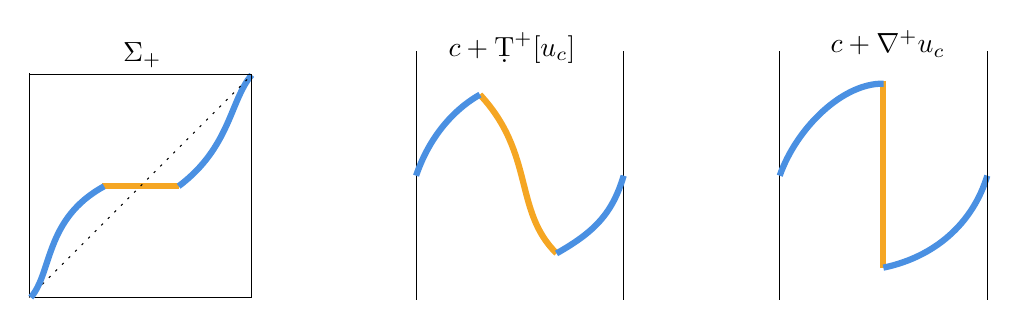
\begin{tikzpicture}[x=0.75pt,y=0.75pt,yscale=-0.8,xscale=0.8]

  \draw [color={rgb, 255:red, 245; green, 166; blue, 35 }  ,draw opacity=1 ][line width=2.25]    (547.4,51) -- (547.4,163.6) ;
  \draw [color={rgb, 255:red, 74; green, 144; blue, 226 }  ,draw opacity=1 ][line width=2.25]    (547.4,163.6) .. controls (578.2,157.2) and (601.2,137.2) .. (610,108.2) ;
  \draw [color={rgb, 255:red, 245; green, 166; blue, 35 }  ,draw opacity=1 ][line width=2.25]    (77,114.53) -- (123,114.53) ;
  \draw [color={rgb, 255:red, 74; green, 144; blue, 226 }  ,draw opacity=1 ][line width=2.25]    (123,114.53) .. controls (154.2,91.2) and (154,62.53) .. (167,47.53) ;
  \draw    (485,33.4) -- (485,183) ;
  \draw    (610,33.4) -- (610,183) ;
  \draw    (266,33.4) -- (266,183) ;
  \draw    (391,33.4) -- (391,183) ;
  \draw    (33,46.4) -- (33,181.53) ;
  \draw    (167,47.53) -- (167,181.53) ;
  \draw    (33.95,181.53) -- (167,181.53) ;
  \draw    (32.85,47.53) -- (167,47.53) ;
  \draw [color={rgb, 255:red, 245; green, 166; blue, 35 }  ,draw opacity=1 ][line width=2.25]    (304.45,59.4) .. controls (337.6,95) and (324.6,129.4) .. (350.6,155) ;
  \draw  [dash pattern={on 0.84pt off 2.51pt}]  (33,181.53) -- (167,47.53) ;
  \draw [color={rgb, 255:red, 74; green, 144; blue, 226 }  ,draw opacity=1 ][line width=2.25]    (485,108.2) .. controls (495.2,79.2) and (523.2,52.2) .. (547.6,52.8) ;
  \draw [color={rgb, 255:red, 74; green, 144; blue, 226 }  ,draw opacity=1 ][line width=2.25]    (350.6,155) .. controls (373.2,142.2) and (384.2,131.2) .. (391,108.2) ;
  \draw [color={rgb, 255:red, 74; green, 144; blue, 226 }  ,draw opacity=1 ][line width=2.25]    (266,108.2) .. controls (275.2,81.2) and (292.2,66.2) .. (304.45,59.4) ;
  \draw [color={rgb, 255:red, 74; green, 144; blue, 226 }  ,draw opacity=1 ][line width=2.25]    (78.09,114.62) .. controls (42.2,134.2) and (46.98,166.56) .. (33.95,181.53) ;

  % Text Node
  \draw (88,26.4) node [anchor=north west][inner sep=0.75pt]    {$\Sigma _{+}$};
  % Text Node
  \draw (284,20.4) node [anchor=north west][inner sep=0.75pt]    {$c+\d T^{+}[ u_c]$};
  % Text Node
  \draw (514,19.4) node [anchor=north west][inner sep=0.75pt]    {$c+\nabla ^{+} u_c$};



\end{tikzpicture}

\end{document}